\chapter{Reconstruction, Cleaning and Analysis Techniques}
\label{ch:reconstruction}
\begin{flushright}
\textit{Shall I refuse my dinner because I do not fully understand the process of digestion? $\sim$ Oliver Heaviside}
\end{flushright}
Because the in-ice IceCube detector is sparsely distributed, it is not straightforward to unambiguously reconstruct the particle (interactions). The scattering and absorption of photons, tilt of ice sheets, bubble column, etc. lead to uncertainties and make reconstruction challenging. Over the years, multiple reconstruction methods have been developed in the collaboration. They range from very fast (and simple) reconstructions, necessary for online filtering, to slow (and more refined) ones. Multiple reconstruction algorithms have been used in this analysis and are explained in more detail in this chapter.

\section{Reconstruction}

\subsection{Likelihood}
Reconstruction algorithms usually have no unique solutions to describe the set of measured values of an event. The likelihood $\mathcal{L}(\vec{x} |\vec{a})$ describes the probability of a set of parameters ${\vec{a}}$ to be expressed in a set of experimentally measured values ${\vec{x}}$. The parameters, ${\vec{a}}$, typically define the particle's characteristics (energy, direction, position, type, etc.) while the measured values ${\vec{x}}$ are determined from the detector response (number of PE, timing, position of hit DOMs, etc.). This likelihood is equal to the cumulative probability

\begin{equation}
\mathcal{L}(\vec{x}|\vec{a}) = \prod_i p(x_i|\vec{a}),
\end{equation}
\noindent where $p(x,\vec{a})$ is the probability that we measure a certain value $x$ from a set of independent values $\vec{x}$ given an initial set of parameters $\vec{a}$. The best possible guess for the unknown parameters $\vec{a}$ is the most likely set that will result into the experimental values. This is done by maximizing the likelihood $\mathcal{L}$. The reconstruction algorithms below rely on analyzing parameters that assume a single, long track

\begin{equation}
\label{eq:vec}
\vec{a} = (\vec{r_0},t_0,\vec{p},E_0),
\end{equation}
\noindent where $\vec{r_0}$ is the position vector of the particle at a time $t_0$ with a direction $\vec{p}$ and initial energy $E_0$. 

\subsection{\texttt{Line-Fit}}
\label{subsec:lf}

\begin{figure}
\centering
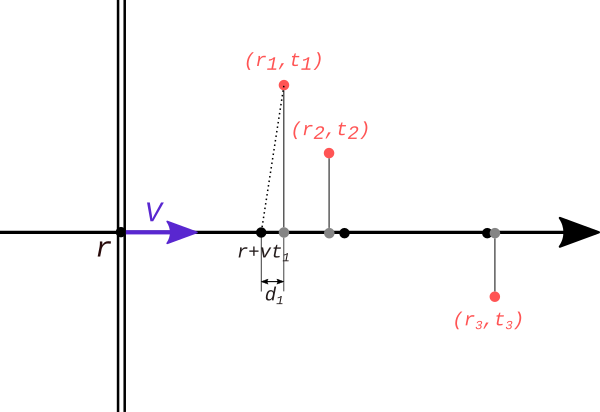
\includegraphics[width=0.6\textwidth]{chapter7/img/linefit.png}
\caption{Figure illustrating how \texttt{LineFit} works. The position, $\vec{r}$, and velocity, $\vec{v}_\textrm{part}$ minimizing the distance of the DOMs to the track is calculated. The dotted line is one of the distances that is minimized in Eq. \ref{eq:lf}.}
\label{fig:lf}
\end{figure}

\noindent One of the most simple approaches in constructing a parameter profile is by calculating the track that, overall, has the closest approach of all the hit optical modules and is called \texttt{Line-Fit}\index{Line-Fit} (LF) \cite{Ahrens:2003fg}. If we assume that a particle starts at a position $\vec{r}$ at a time 0 and travels at a velocity of $\vec{v}_\textrm{part}$, then its position at any given time is

\begin{equation}
\vec{r'} = \vec{r} + \vec{v}_{\textrm{part}}t.
\end{equation}

\noindent We want to calculate the best possible estimate of the velocity $\vec{v}_\textrm{part}$ and an initial position $\vec{r}$. Each DOM has a known location, $\vec{r}_i$, and measured time of a pulse, $t_i$. In this algorithm one assumes that a wavefront perpendicular to the particle's direction is traveling along with the particle. If the veloctity $\vec{v}_\textrm{part}$ is fixed, then the position of the particle at later times is known (black points in Fig. \ref{fig:lf}). However, the Cherenkov wavefront should be set at an angle and because scattering, PMT jitter, noise, etc. are not taken into account, this will not agree with the DOM position projected along the particle path (grey dots). The unknown velocity $\vec{v}_\textrm{part}$ and position $\vec{r}$ are the analytical solutions after minimizing the distances $d_i$ as shown in the figure\footnote{Minimizing $r_i - r'$ (dotted line in Fig. \ref{fig:lf}) is the same as minimizing $d$.}

\begin{equation}
\label{eq:lf}
\begin{split}
S(\vec{r},\vec{v}_{\textrm{part}}) &\equiv \sum^{N_{\textrm{hit}}}_{i=1} \rho(\vec{r},\vec{v}_\textrm{part},\vec{r}_i,t_i)^2\\
&= \sum^{N_{\textrm{hit}}}_{i=1} \left(\vec{r}_i - \vec{r} - \vec{v}_\textrm{part}t_i \right)^2,
\end{split}
\end{equation}
\noindent where $N_\textrm{hit}$ are the number of pulse hits. The analytical solution by minimizing this equation is equal to

\begin{equation}
\vec{r} = \langle\vec{r}_i\rangle - \vec{v}_\textrm{part}\langle t_i\rangle \ \ \ \textrm{and}\ \ \ \vec{v}_\textrm{part} = \frac{\langle \vec{r}_i t_i\rangle - \langle \vec{r}_i \rangle \langle t_i \rangle }{\langle t_i^2 \rangle - \langle t_i \rangle^2},
\end{equation}
\noindent where $\langle x \rangle$ denotes the average of a parameter $x$ over all hits $i$.

Because this is an analytical equation, this algorithm is very fast and therefore often used in online processing.
 
\subsubsection{\texttt{Improved Line-Fit}}
While disregarding the Cherenkov profile is inherent to the simplified LF model for computational reasons, removing hits generated by photons that scattered for a significant length of time will mitigate the effect of ignoring the photon scattering in the ice. It was found that a basic filter could identify these scattered hits, and improve accuracy by almost a factor of two by removing them from the dataset. More formally, for each hit $h_i$, the algorithm looks at all neighboring hits within a neighborhood of $\mu$, and if there exists a neighboring hit $h_j$ with a time stamp that is $t$ earlier than $h_i$, then $h_i$ is considered a scattered hit, and is not used in the basic reconstruction algorithm. Optimal values of $\mu$ and $t$ were found to be 156 m and 778 ns by tuning them on simulated muon data \cite{Aartsen:2013bfa}.\\

\noindent This ``delay cleaning'' is done by computing the Huberfit on the remaining data points and minimizing

\begin{equation}
\sum^{N_{\textrm{hit}}}_{i=1} \phi(\rho(\vec{r},\vec{v}_\textrm{part},\vec{r}_i,t_i)),
\end{equation}
\noindent where $\rho$ is defined in Eq. \ref{eq:lf} and the Huber penalty function $\phi$ is defined as

\begin{equation}
\phi(\rho) \equiv \left\{
    \begin{array}{ll}
        \rho^2 &\textrm{if } \rho < \mu \\
        \mu\left(2\rho - \mu\right) & \textrm{if }\rho \geq \mu
    \end{array}
    \right.
    .
\end{equation}
\noindent Because of the overal performance increase of this method, all LF computations were done with the improved version (although still often referred to as ``Line-Fit'').

\subsection{SPE and MPE}
\label{subsec:spempe}
A more intricate method of track reconstruction is done by taking the geometrical shape of the Cherenkov cone into account and relying on simulation fits where a seed track is implemented (usually from the fast \texttt{Line-Fit} algorithm).


\begin{figure}
\centering
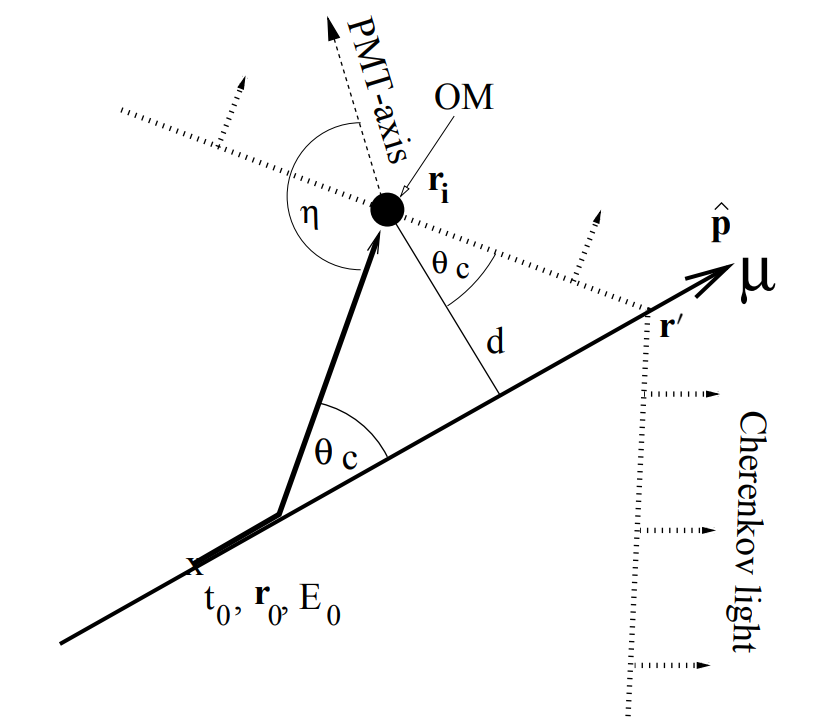
\includegraphics[width=0.6\textwidth]{chapter7/img/reconstruction.png}
\caption{Figure illustrating a muon track passing close by an optical module and defining the parameters used in the reconstruction algorithms. Illustration from Ref. \cite{Ahrens:2003fg}.}
\label{fig:reconstruction}
\end{figure}

Let us assume a particle is traveling close to a DOM with parameters defined in Eq. \ref{eq:vec} as illustrated in Fig. \ref{fig:reconstruction}. The minimal distance of the track to the DOM is equal to $d$ and the PMT-axis (downwards relative to DOM) has an angle offset of $\eta$ degrees of the Cherenkov wave direction. In perfect conditions, the \textit{time residual} (time between the observed hit time and the ``expected'' time ) is a delta function centered around 0, where

\begin{equation}
t_{\textrm{res}} \equiv t_{\textrm{hit}} - t_{\textrm{geo}},
\end{equation}
\noindent with

\begin{equation}
t_\textrm{geo} = t_0 + \frac{\vec{p} \cdot (\vec{r}_i - \vec{r}_0) + d\cdot \tan (\theta_c)}{c_\textrm{vac}},
\end{equation}
\noindent which is equal to the time of the particle to travel from the position $\vec{r}_0$ to $\vec{r}'$ as illustrated in the figure. The accompanying Cherenkov wavefront that sent out photons at a time $t_0$ from $\vec{r}_0$ will cross the DOM when the particle is at a position $\vec{r}'$. Due to noise effects, PMT jitter, light from secondary interactions, DOM orientation, etc. the time risidual is smeared and shifted. The p.d.f. was estimated with photon simulations in ice and fitted to a Pandel function \cite{Ahrens:2003fg}. The time likelihood profile for single photons $i$ at the locations of the hit DOMs is then

\begin{equation}
\mathcal{L}_\textrm{time} = \sum^{N_\textrm{hit}}_{i=1} p_1 (t_\textrm{res} | \vec{a} = {d_i,\eta_i,...}).
\end{equation}
\noindent An initial particle position and direction are found by maximizing the likelihood and iterated a couple of times to find the global maximum instead of a local. This fitting is called the Single PhotoElectron (SPE)\index{SPE} fit.\\

\noindent The description of single photons arriving at the optical modules cannot be correct since electrical and optical signal channels can only resolve multiple photons separated by a few 100 ns and $\approx$ 10 ns, respectively. In the Multi-PhotoElectron (MPE) fit, one accounts for the fact that the early photons in a DOM hit scattered less in the ice. The p.d.f. for the first photon out of a total of $N$ to arrive with a time residual of $t_\textrm{res}$ is

\begin{equation}
p^1_N (t_\textrm{res}) = N \cdot p_1(t_\textrm{res}) \cdot \left(\int^\infty_{t_\textrm{res}} p_1(t) dt \right)^{(N-1)} = N \cdot p_1 (t_\textrm{res}) \cdot (1-P_1 (t_\textrm{res}))^{(N-1)},
\end{equation}
\noindent where $P_1$ is the cumulative distribution of the single photon p.d.f..
\subsection{\texttt{Millipede}}
\label{subsec:millipede}
To have a better handle on the particle energy and cascades along the track, the module \texttt{Millipede} was developed. The number of photons seen at each optical module depends on multiple factors that were mentioned throughout this text, such as the ice characteristics, timing, etc. In this module, the expected number of photons is said to depend on the energy that was deposited along a track and a \textit{light yield factor} that depends on the DOM position and the location of emission

\begin{equation}
\label{eq:n_exp}
\begin{split}
N_{\textrm{exp},k} &= \rho_k + \sum^n_{i=1} \Lambda(\vec{r}_k,\vec{r}_i') E_i\\
&= \rho_k + \vec{\Lambda}(\vec{r}_k,\vec{r}_i') \cdot \vec{E},
\end{split}
\end{equation}
where $k$ refers to a certain DOM and $i$ refers to a certain energy deposit such as illustrated in Fig. \ref{fig:millipede}.

\begin{figure}
\centering
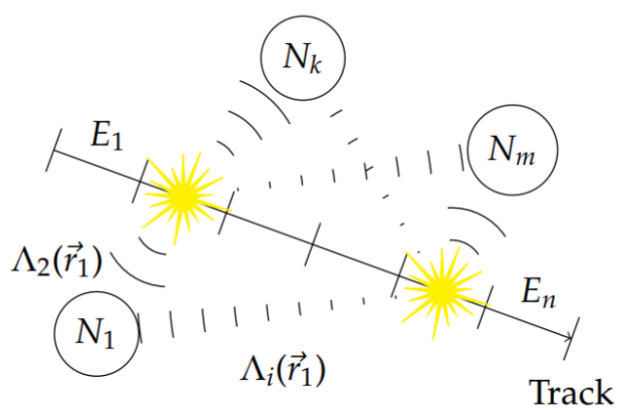
\includegraphics[width=0.6\textwidth]{chapter7/img/millipede.png}
\caption{Illustration of the working principles of the \texttt{Millipede} toolkit. A track is subdivided into segments that each deposit a certain energy, $E_i$. Different segments can contribute to the total number photons seen per DOM, $N_k$.}
\label{fig:millipede}
\end{figure}

The likelihood is assumed to follow a Poisson distribution with a mean equal to the expected amount of photons, $N_{\textrm{exp},k}$

\begin{equation}
\mathcal{L}_k = \frac{\left(\vec{\Lambda} \cdot \vec{E} + \rho_k \right)^{N_{\textrm{seen},k}}}{N_{\textrm{seen},k}!} e^{-\vec{\Lambda} \cdot \vec{E} - \rho_k}.
\end{equation}
\noindent For easier, faster and more accurate computation the logarithm of the likelihood is used

\begin{equation}
\begin{split}
\ln \mathcal{L}_k &= N_{\textrm{seen},k} \ln \left(\rho_k + \sum^n_{i=1} \Lambda(\vec{r}_k,\vec{r}_i') E_i \right) - \ln \left(N_{\textrm{seen},k}!\right) - \sum^n_{i=1} \Lambda(\vec{r}_k,\vec{r}_i') E_i - \rho_k\\
&= N_{\textrm{seen},k} \ln \left(\rho_k + \vec{\Lambda}(\vec{r}_k) \cdot \vec{E} \right) - \vec{\Lambda}(\vec{r}_k) \cdot \vec{E} - \rho_k - \ln\left(N_{\textrm{seen},k}!\right)
\end{split}
\end{equation}
\noindent Maximizing the total likelihood (summing over all $m$ DOMs) with respect to the energy gives 

\begin{equation}
\nabla_{\vec{E}} \ln \mathcal{L} = \nabla_{\vec{E}} \sum^m_{k=1} \ln \mathcal{L}_k = \sum^m_{k=1} \left(\frac{N_{\textrm{seen},k} \vec{\Lambda}(\vec{r}_k)}{\vec{\Lambda}(\vec{r}_k) \cdot \vec{E} + \rho_k} - \vec{\Lambda}(\vec{r}_k) \right) = 0.
\end{equation}
\noindent This equation holds if all terms in the sum vanish, i.e. if for all DOMs holds that

\begin{equation}
\begin{split}
N_{\textrm{seen},k} = &\vec{\Lambda}(\vec{r}_k) \cdot \vec{E} + \rho_k\\
\overset{\textrm{Eq.}\ref{eq:n_exp}}{=} &N_{\textrm{exp},k}
.
\end{split}
\end{equation}
\noindent This can be written in a set of linear equations

\begin{equation}
\vec{N} - \vec{\rho} = \mathbf{\Lambda} \vec{E}, 
\end{equation}
\noindent where

\begin{equation}
\mathbf{\Lambda} = 
\begin{pmatrix}
\Lambda(\vec{r}_1,\vec{r}_1') & \cdots & \Lambda(\vec{r}_1,\vec{r}_n')\\
\vdots  & \ddots & \cdots \\
\Lambda(\vec{r}_m,\vec{r}_1') & \cdots & \Lambda(\vec{r}_m,\vec{r}_n')\\
\end{pmatrix},
\end{equation}
\noindent is the \textit{response matrix} and has to be inverted to find the energies in the vector $\vec{E}$. It describes the DOM response to light output from certain segments along a track. The entries in this matrix come from simulations that produce spline tables. Simplified sources, such as minimum ionizing muons and isotropically emitting point sources are simulated in Monte Carlo simulations at certain discrete points. Interpolation is done using spline functions. More information, such as how timing information can be implemented, can be found in Refs. \cite{millipedeinternal,stefthesis}.

%\section{Event splitting}
%Multiple triggers are combined into one event by the event builder (see Section \ref{subsec:triggers}. The triggerspl

\subsection{\texttt{FiniteReco}}
\label{subsec:finitereco}
\texttt{FiniteReco} is a module that tries to reconstruct if particles are starting, stopping, contained or through-going. The hit DOMs around a seed track are checked to have seen light and the first and last emission points along the track are used to check the possible hypotheses.

Because the edges of the detector are not well defined\footnote{Imagine a cascade 20 m below the lowest DOMs. It is still possible for light to reach the bottom modules of the detector.}, the likelihoods of individual DOMs to have seen a hit lead to a total likelihood that doesn't give a conclusive answer, but the starting and stopping probabilities can be compared to a through-going track hypothesis.
\subsection{\texttt{Paraboloid}}
\label{subsec:paraboloid}

In Sections \ref{subsec:lf} and \ref{subsec:spempe}, we discussed how a particle's direction could be estimated. The \texttt{Paraboloid} module tries to provide an estimate for the error on this direction. A highly energetic muon with hunderds of hit DOMs will lead to a much better directional resolution than a dim track where only a handful of DOMs are hit. In general, the likelihood space around the estimated direction is scanned and compared to the likelihood of the initial track estimation. This method also gives a robust estimation if the initial track direction is in fact located at the global maximum likelihood or a local one. \texttt{Paraboloid} constructs a grid of zenith and azimuth points near the minimum and for each point on the grid it does a three-parameter minimization for the vertex holding the zenith and azimuth constant. The likelihood values for each point on the grid are then fit to paraboloid using a $\chi^2$ minimization since the shape of the log-likelihood space near the minimum should have a paraboloid (2D parabola) shape. Of importance are the parameters of the corresponding error, which is assumed to correspond to an ellipse for the $1\sigma$ contours.\\

\noindent The module computes the lengths of the semimajor and semiminor axes of the $1\sigma$ error ellipse $\sigma_1$ and $\sigma_2$\footnote{The confidence intervals $\sigma_\theta$ and $\sigma_\phi$ can be found by rotating the minor and minor axes $\sigma_1$ and $\sigma_2$. How this is done can be found in the literature, but is of no importance here.}. It was found that the quadratic mean of both uncertanties provides for a good single-valued estimate for the angle uncertainty

\begin{equation}
\label{eq:paraboloid}
\sigma_\textrm{para} = \sqrt{\frac{\sigma_1^2 + \sigma_2^2}{2}}.
\end{equation}

\noindent Since $\sigma_1$ and $\sigma_2$ should follow univariate Gaussian distributions, $\sigma_\textrm{para}$ will be the radius parameter in a bivariate distribution, meaning that the mean should be set to $1.177\sigma$\footnote{The CDF of the Rayleigh distribution $1-e^{-x^2/2\sigma^2}$ is equal to the containment for a bivariate normal distribution. Implementing $x=1.177\sigma$ yields a factor of 0.5.}. This means, that if we calculate the great circle distance between the MC truth of the signal particle with the reconstruction direction and divide it with $\sigma_\textrm{para}$, the distribution should peak at 1.177 (mean). This variable is called the \textit{paraboloid pull} and should be compared to an energy related variable (here the number of hit DOMs (NCh) is used). In Fig. \ref{fig:paraboloidpull}, it is clear that there is an offset, which is seen in all analyses, that can be explained by multiple factors in Monte Carlo simulations but mainly stems from our incomplete knowledge and non-perfect simulations of the ice.

\begin{figure}[t]
\centering
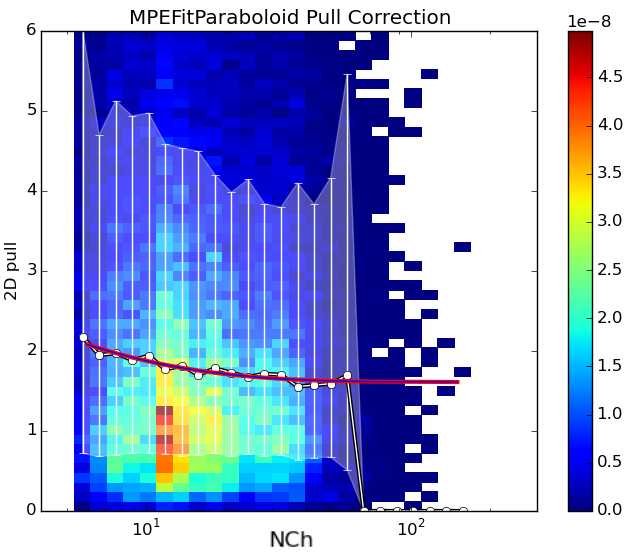
\includegraphics[width=0.48\textwidth]{chapter7/img/pullbeforecorrection.png}
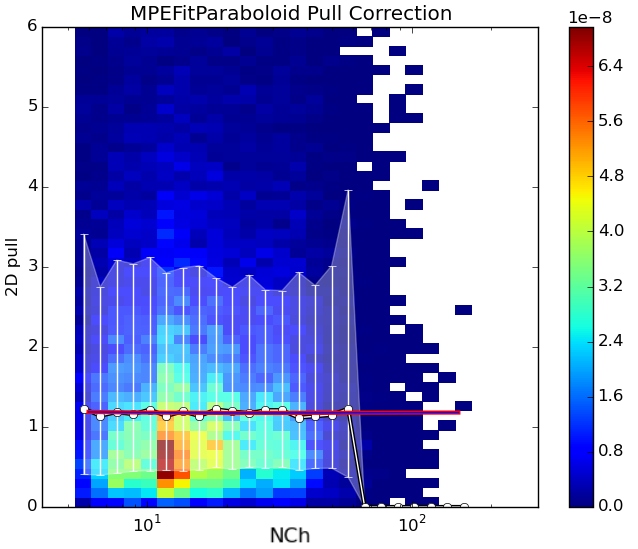
\includegraphics[width=0.48\textwidth]{chapter7/img/pullaftercorrection.png}
\caption{\textit{Left: }Paraboloid pull in function of the number of hit DOMs shows that the global average (red/purple line) is not centered at 1.177. \textit{Right: }Pull after correction.}
\label{fig:paraboloidpull}
\end{figure}

More information can be found in Ref. \cite{Neunhoffer:2004ha}.

\section{Pulse cleaning}
\label{sec:pulsecleaning}
As explained in Section \ref{subsec:calibration}, each DOM in IceCube has an intrinsic noise rate. This dark noise is observed in every triggered event and seen as random hits in the detector added to the hit pattern of tracks and cascades. These spurious hits are a large nuisance factor in event reconstructions, leading to misidentification and errors in the result. Noise cleaning should be done in early stages of event processing and analysis to reduce a large rate of bad reconstructed events that pass cut selections. One of the most conservative ways is to only look at HLC hits (\textit{HLC cleaning}), but is too demanding for most low-energetic events that will have multiple hits from isolated DOMs. 

Another, more conservative method, is the \texttt{seededRT} \index{seededRT} algorithm. This method relies on the ``$RT$-cut'', which was already implemented in the time of AMANDA operations. $R$ is a designed radius and $T$ refers to the time between multiple possible pulse times (e.g. the pulse of one DOM starts during the time window of a second DOM's pulse, or stops during the time window). The full description can be found in Ref. \cite{RTcutwiki}, but can be summarized as follows: DOMs are required to be in a temporal and spacial coincidence that is physically possible (e.g. signal between DOMs cannot exceed the speed of light in vacuum). This method is however computationally expensive since all DOM pairs have to be looped over\footnote{The number of pairs for $n$ DOMs is equal to $\frac{1}{2}n(n-1)$ and scales with $n^2$.}. The \texttt{seededRT} algorithm takes a subset of seeds that are considered to be mostly signal related hits. These seeds can be provided by, for example, using HLC information. By adding all further hits found within the seed's $RT$-range to the list of seed hits and iterating until a convergence, only those (SLC) hits are kept that cluster around the initial seed hits. Outlying noise hits are supposedly not added and thus removed in the cleaned output. This method does not scale as drastically as the original $RT$-cut method.


\section{\texttt{IceHive}}
\label{sec:icehive}
In Section \ref{subsec:triggers}, it was explained how multiple triggers were combined into one global trigger. In a first step, Q-frames are simply re-split into the individual events that belong to the different subtriggers. In about 15\% of cases the data read out in one of these P-frames contains more than one primary interaction. This pile-up effect is referred to as \textit{coincident events}\index{coincident events}. It is a direct result of the traversal time of a couple of microseconds in the detector\footnote{The speed of light in vacuum is equal to $\approx$ 0.3 m/ns, meaning the particle travels around 100 m in 0.3 $\mu$s, without accounting for the delayed photon propagation necessary for detection.}, the large flux of low-energetic events and the trigger time windows of a couple of microseconds. This can be problematic for reconstructions, as can be seen in Fig. \ref{fig:coincidentevent} where two downgoing muons can be reconstructed as an upgoing track.\\

\begin{figure}[t]
\centering
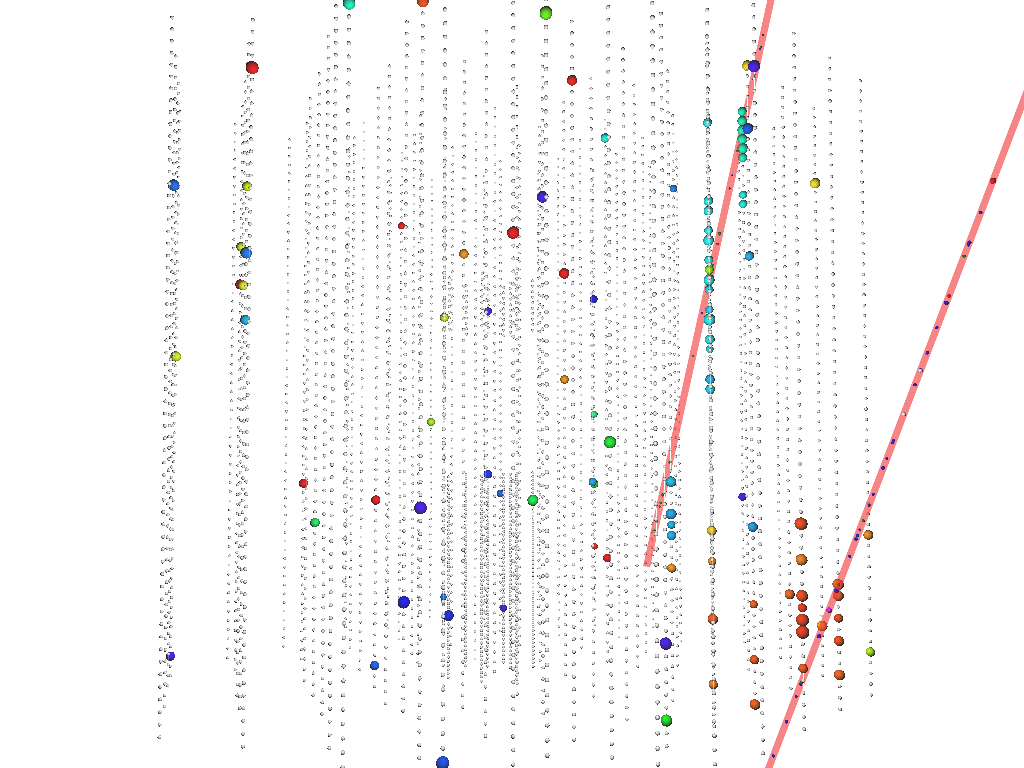
\includegraphics[width=0.8\textwidth]{chapter7/img/coincidenteventsCORS.png}
\caption{Event display of a simulated coincident event of two downgoing muons. The colors of the event range from red (early) to blue (late). The first muon hits the bottom of the detector, while the second traverses mainly the upper part. These events are often reconstructed as a single up-going event and therefore result in a large background contribution. The scattered isolated hits are due to noise effects and mostly removed by pulse cleaning.}
\label{fig:coincidentevent}
\end{figure}

\noindent There are two modules that try to clean events more thoroughly than pulse cleaning alone. The first is \texttt{TopolocalSplitter}\index{TopologicalSplitter} (TS), which starts from the Q-frames and loops over pulses and splits the event into clusters of pulses that contain at least a number of causally\footnote{The time between two DOM hits cannot be less than the time that light may have taken.} connected pulses within a certain time window. Some extra cleaning, similar to \texttt{seededRT} cleaning, is done in addition and can split coincident events that have overlapping readout windows, but are geometrically separated.

The second module, and also used in this analysis, is called \texttt{IceHive}. A full description can be found in the doctoral thesis of M. Zoll \cite{mzollthesis}. The module consists of two main parts: one that splits events and handles coincident events, \texttt{HiveSplitter}, and another that has a refined pulse cleaning, \texttt{HiveCleaning}.

\subsection{\texttt{HiveSplitter}}
The module assumes that individual particles will create \textit{clusters} of hits in the detector. A cluster can grow within a certain time window, but is separated from another cluster if it's not spatially connected. An initial cluster is formed if the multiplicity of hits exceeds a certain threshold (usually 3 or 4). The main difference in this module versus \texttt{TopologicalSplitter} is that it uses hexagons to describe the detector instead of assuming a spherical parameterization. It makes more sense to optimize the search volume, where hits are clustered together, with a shape that describes the detector well and uses a discrete spacing between larger volumes instead of a uniformly growing sphere. The hexagonal shape is set by defining three heights. The first height is defined along the string of the hit DOM and is equal to the vertical distance along the string. The second height is the vertical height along the neighboring strings. The third hight is the vertical height along the next-to-neighboring strings. An example is shown in Fig. \ref{fig:hexagon}.

\begin{figure}[t]
\centering
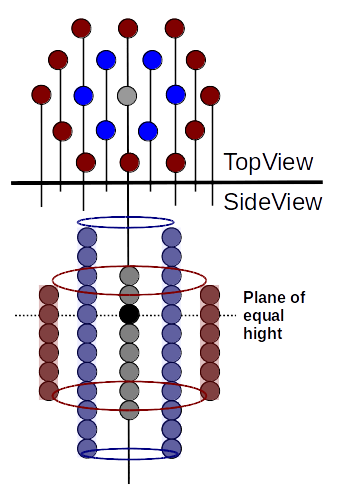
\includegraphics[width=0.5\textwidth]{chapter7/img/hexagons.png}
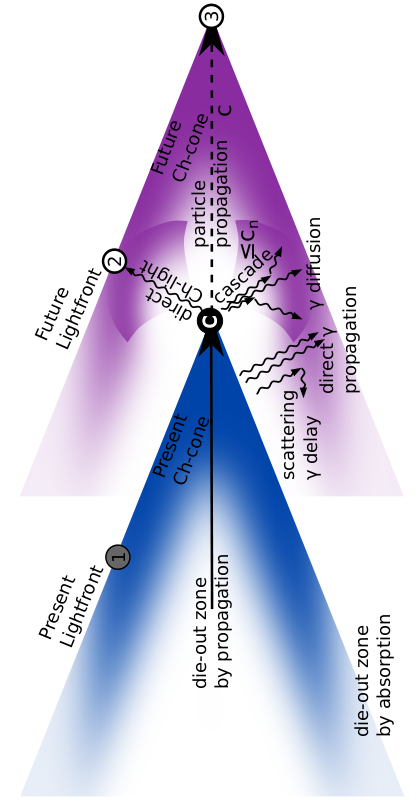
\includegraphics[width=0.4\textwidth]{chapter7/img/cherenkovzoll.png}
\caption{\textit{Left: }The black circle illustrates a DOM that triggered a hit in the detector. The grey circles symbolize the DOMs along the string of the hit DOM. The number of DOMs that can be included in the active volume depends on the height defined by the module. The blue/purple DOMs belong to the neighboring strings and the red/brown DOMs to the next-to-neighboring strings. The heights of both these sets of DOMs are also set by the module. This example shows $h_2 > h_1 > h_3$, the heights are also asymmetric in this example. \textit{Right: }Illustration of Cherenkov emission profile of a traversing particle. Both figures from Ref. \cite{mzollthesis}.}
\label{fig:hexagon}
\end{figure}
When the active region is set, there is an additional check to see if DOMs can be ``connected''. \texttt{IceHive} assumes certain emission profiles (for both cascades as tracks) where light is produced. Three possible connections are assumed:

\begin{enumerate}
\item Hits occur at the same time, but at a spatial distance in agreement with the Cherenkov emission profile (hits C\&1 and 2\&3 in Fig. \ref{fig:hexagon}).
\item Hits occur at a different time and a different location, but in agreement with the Cherenkov emission profile (hits C\&2 in Fig. \ref{fig:hexagon}).
\item Hits on topologically identical sites of an emission pattern that has moved along with the propagation of the particle (hits C\&3 and hits 1\&2 on Fig. \ref{fig:hexagon}).
\end{enumerate}
These clusters are finally separated into different P-frames and thus regarded as distinct events.

\subsection{\texttt{HiveCleaning}}
Additionally, a similar cleaning as explained in Section \ref{sec:pulsecleaning} can be performed. Isolated hits that do not have neighboring hits occurring within a certain distance and time window, are removed. The main difference between this and \texttt{seededRT} cleaning is that the module again uses the hexagons as defined in the previous section.\\

\subsection{Remark}
\noindent The usage of \texttt{IceHive} has a great performance in separating coincident events, but often ``overperforms'' and splits clusters of hits that are originating from the same particle. This is predominantly the case for dim tracks that have large separations in between clusters (most of the triggered SMP events are of this type). It is because of this that the module \texttt{CoincSuite} \index{CoincSuite} was designed.

\section{CoincSuite}
\begin{figure}[t]
\centering
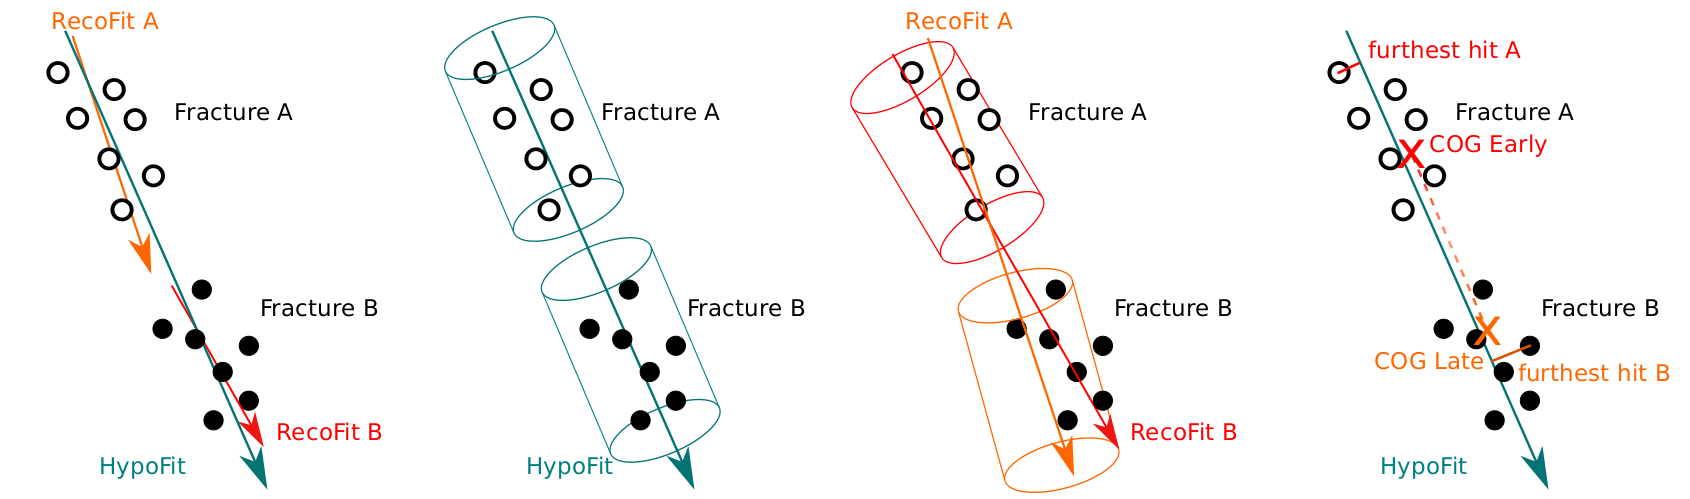
\includegraphics[width=\textwidth]{chapter7/img/coincsuite.png}
\caption{Schematic illustrations of possible recombination scenarios with the \texttt{CoincSuite} module. Two events are compared to each other or the combined event (HypoFit) in several different ways.}
\label{fig:coincsuite}
\end{figure}
Several testing algorithms allow to check if two or more split P-frames can originate from a single event. Five different scenarios were tested in this analysis, the first four are also chronologically shown in Fig. \ref{fig:coincsuite}:
\vspace{2mm}

\begin{enumerate}
\item Cluster alignment: the reconstructed direction of the individual clusters is compared to the direction of a reconstruction that uses the combined hits (HypoFit). The directions should be within a certain criticle angle.
\item Cylinder cluster containment: the DOMs of the individual clusters should be able to be grouped together in a cylinder that has its center and direction along the HypoFit.
\item Cylinder cluster alignment: a cylinder around the reconstruction of each cluster is draw. The cylinders should overlap within a certain fraction.
\item COG\footnote{Similar to COM (Center Of Mass), the COG is a weighted average position of the hit DOMs. DOMs that register more light get a heigher weight.} connection: the second quarter of the COG of the first cluster and the third quarter of the COG of the second cluster are computed. These COG should lie close enough and have to be in the vicinity of the HypoFit.
\item Velocity test: tests if the velocity of the HypoFit is close to the speed of light.
\end{enumerate}

\vspace{2mm}
\noindent The combination of \texttt{IceHive}, which does a very good job in cleaning events, but often overperformes and splits events that shouldn't be, and \texttt{CoincSuite}, which recombines events that were wrongfully split, leads to a very powerful tool to clean events.

\section{Analysis techniques}
\textcolor{red}{Komt hier iets dat je gebruikt in het volgende hoofdstuk maar nog niet hebt uitgelegd?}
\section{Boosted Decision Tree classifiers}
\label{sec:BDT}
Given a certain event with a fixed set of variables that are constructed in an analysis, the question remains if the event is in fact a \textit{signal} or \textit{background} event. One can rely on Monte Carlo simulations to get a handle on the variable distribution in both sets. The most general and still widely used method is to use a cut-and-count approach where a cut is placed on a certain variable that discards events that fail the requirement. A Boosted Decision Tree (BDT) inspects a set of set variables and classifies an event with a score that ranges from -1 to 1. The higher the score, the more an event is regarded as signal-like. How this is done is given in more detail below. Boosted decision trees rely on multiple individual trees. Therefore, we will first explain how a single tree classification works.


\subsection{Stucture}
The goal of a decision tree is to determine if an event is signal- or background like. It uses a tree-like structure where certain selection criteria are used at different nodes as illustrated in Fig. \ref{fig:bdt}.

\begin{figure}[t]
\centering
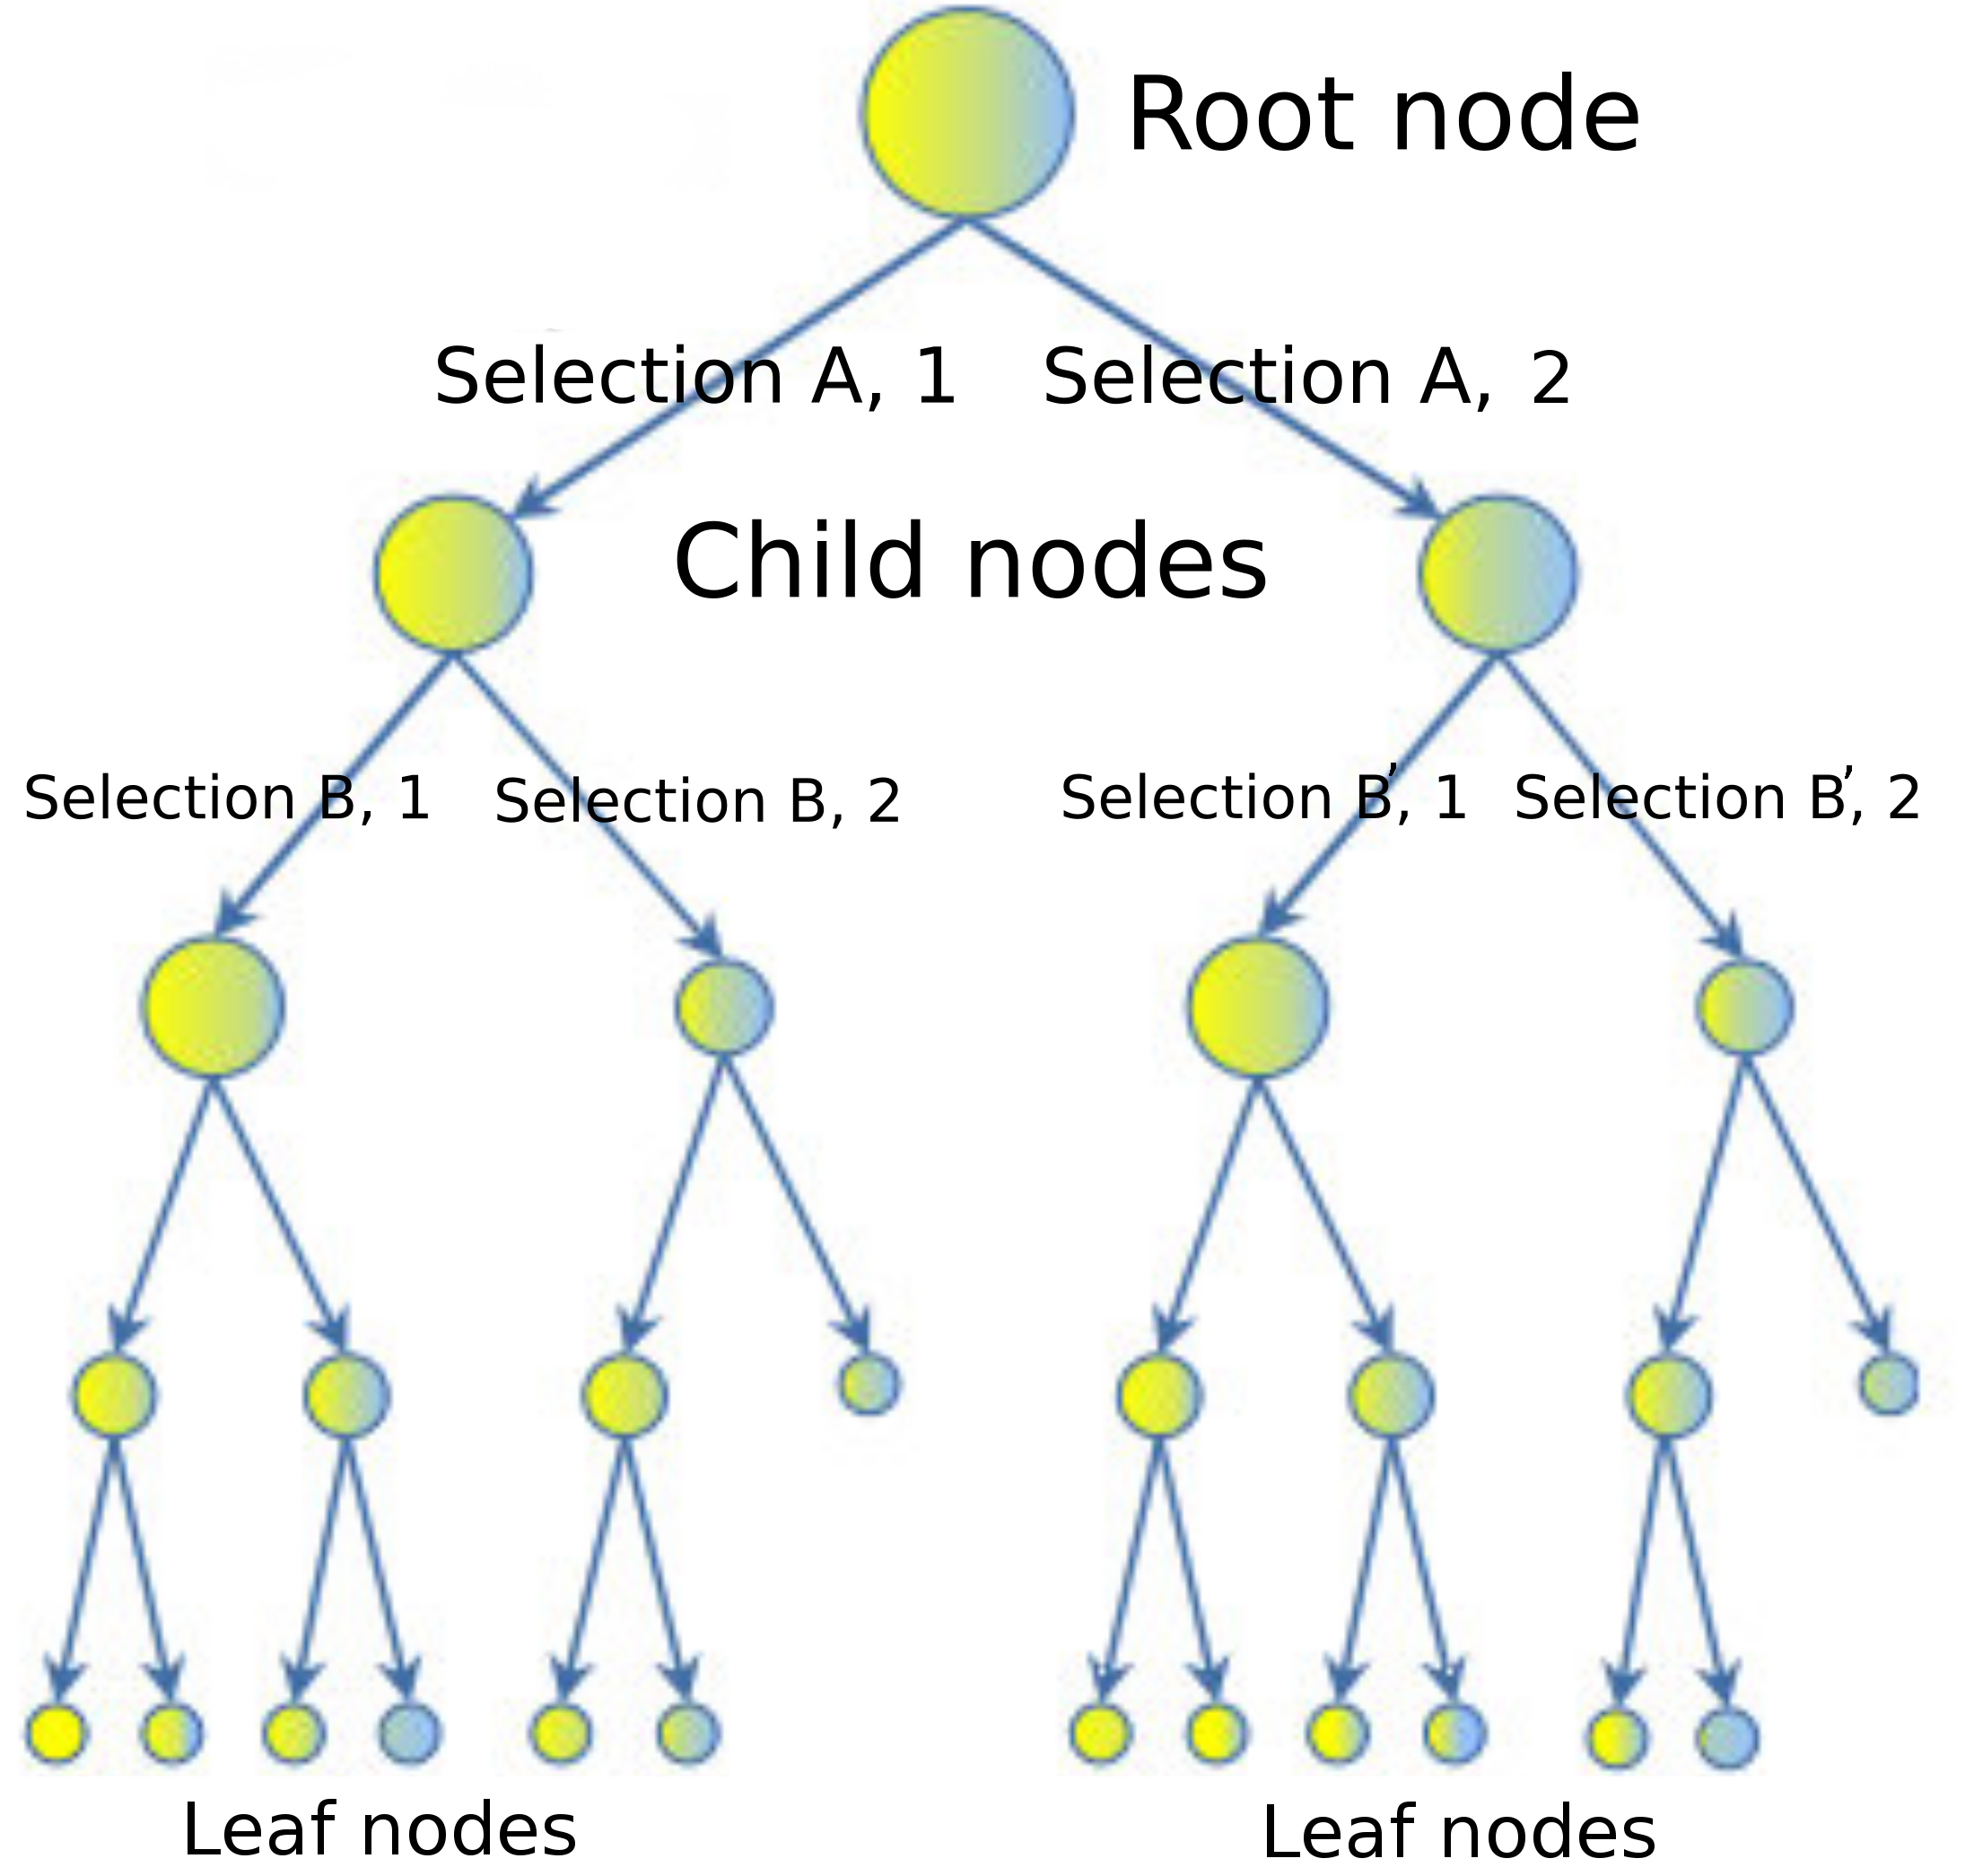
\includegraphics[width=0.5\textwidth]{chapter7/img/bdt.png}
\caption{Illustration of decision tree scheme. Selection B and B' denote a selection on the same variable, but other requirement.}
\label{fig:bdt}
\end{figure}
A decision tree is a binary tree that places an event into a certain node depending on the selection at a node. The depth of a decision tree can be arbitrarily long, but is determined by a set of criteria defined in Section \ref{subsec:training}. An event consists of a certain set of variables $X = {x_1,x_2,...x_n}$ that are used in the classification. Before any selection criteria, the event is said to be represented by the \textit{root node}. A binary selection then determines to which \textit{child node} the event should be classified, for example: 

\begin{equation}
\begin{split}
\textrm{Selection A} &= x_1 > y_1 \ \ (\textrm{option 1})\\
&= x_1 \leq y_1 \ \ (\textrm{option 2}),
\end{split}
\end{equation}
where $y_1$ is the cut value for variable $x_1$. Similarly, the other selections deterimine where the event is eventually placed. The last nodes are referred to as \textit{leaf nodes} and hold the probabilities of whether an event is more signal- or background-like. These probabilities are translated into a score ranging between -1 (background) and 1 (signal). 

\subsection{Training}
\label{subsec:training}
To construct a decision tree, one first has to ``train'' the algorithm. Given a certain ``signal set'' and ``background set'', all variables used in the BDT are histogrammed and at each bin for each variable the ``best cut'' is set at the first node selection. To determine the optimal cut, we first define the purity of a node, $p$, by

\begin{equation}
p = \frac{\sum_s w_s}{\sum_s w_s + \sum_b w_b},
\end{equation}
\noindent where $w_s$ and $w_b$ refer to the weights of the signal and background events and the Gini index, g,

\begin{equation}
g(p) = p(1-p), 
\end{equation}
is used as a separation variable in this work\footnote{Other possible separation variables include the cross entropy $-p \cdot \ln(p)-(1-p) \cdot \ln(1-p)$ or the misclassification error $1-\textrm{max}(p,1-p)$}. Using the Gini index, the separation gain determines the effectiveness of the cut

\begin{equation}
\label{eq:separationgain}
\Delta S = g_p \cdot \sum w_p - \left(g_l \cdot \sum w_l + g_r \cdot \sum w_r\right),
\end{equation}
\noindent where $g_p$ and $w_p$ denote the Gini index and weights of the parent nodes and similarly for the left and right child nodes. The cut that gives the highest separation gain is subsequently selected. The algorithm stops when one of the following criteria is met:
\vspace{2mm}

\begin{itemize}
\item a node only consists of signal or background events;
\item a certain predefined maximal depth is reached;
\item splitting would cause a child node to have less than a predefined minimal amount of events left;  
\end{itemize}
\vspace{2mm}
and therefore determines the size of a tree. These selection criteria are necessary to avoid overtraining (see Section \ref{subsec:overtraining}).

\subsection{Boosting}
\label{subsec:boosting}
As already implied in the text above, a BDT consists of a \textit{forest} of decision trees. A user specified number of individual decision trees are trained sequentially, with a boosting process in between each training. Boosting consists of adjusting the weights of individual events according to whether the previously trained tree classifies them correctly. In this work, the AdaBoost\footnote{Short for Adaptive Boosting.} algorithm was used for boosting in which the score of an event is a weighted average of the scores the event receives from each tree in the forest \cite{FREUND1997119}.

A BDT may informally be called a ``boosted decision tree'', but it must be understood that there are actually many trees (typically hundreds), and that boosting is a process that occurs between the training of consecutive trees. The approach makes use of the power of numbers: many weak single decision trees combined can be more powerful than one very good decision tree. In general, boosting follows the following steps:
\vspace{2mm}

\begin{enumerate}
\item Train a weak model on training data.
\item Compute the error of the model on each training example.
\item Give higher importance to examples on which the model made mistakes.
\item Re-train the model using ``importance weighted'' training examples.
\item Go back to step 2.
\end{enumerate}
\vspace{2mm}
An example is given in Appendix \ref{ch:adaboostappendix}.\\
\newline
\noindent If $I(s,y)$ is a function equal to 0 when, after tree classification, the sample test score, $s$, is equal to its true identity, $y$, then the error rate for a tree is equal to

\begin{equation}
\epsilon = \frac{\sum_i w_i I(s,y)}{\sum_i w_i}.
\end{equation}
\noindent The boosting factor for the tree is defined as

\begin{equation}
\label{eq:boostfactor}
\alpha = \beta \cdot \ln\left(\frac{1-\epsilon}{\epsilon}\right),
\end{equation}
\noindent with $\beta$ a user defined \textit{boosting beta} and changes the weight of the tree to

\begin{equation}
\begin{split}
w' = w \cdot \exp(\alpha), \ \ \ \ \ \ \ \ \ \ \ \ \ \ \ \ \ \ \ \ \ w' = w \cdot \exp(-\alpha)\\
\textrm{ (correct classification)} \ \ \ \ \textrm{ (incorrect classification),}
\end{split}
\end{equation}
\noindent after which the weights are renormalized so that $\sum w' = 1$. The process is repeated until the number of predefined trees is reached.

Due to its definition, the boost factor $\alpha$ will give good classifiers (which have low error rates) large boost factors. Events that are misclassified are then given larger weights, making the algorithm more likely to classify them correctly in the subsequent tree classifier.

Once the entire BDT is trained, the events can be given a score based on the multiple tree classifiers. This is done by taking the weighted average of all the scores in the individual tree classifiers, using its boost factor $\alpha$ as the weight of the tree. The score of an event $i$ is then given by

\begin{equation}
s_i = \frac{\sum_m \alpha_m \cdot s_{i,m}}{\sum \alpha_m},
\end{equation}
\noindent where we loop over the individual trees denoted with index $m$.

\subsection{Overtraining}
\label{subsec:overtraining}
BDTs are very powerful tools, but if not used correctly could lead to problems that are not easy to spot at first sight. Assume we train our BDT with a certain signal set and background set. If the BDT is trained up to the point of classifying statistical fluctuations, there is said to be \textit{training sample overtraining}. An illustrative example is given in Fig. \ref{fig:overtraining}. Another example is data/MC overtraining. The former can be dealt with with the use of \textit{pruning}, while the latter should show clear data/MC agreement. 

\begin{figure}[t]
\centering
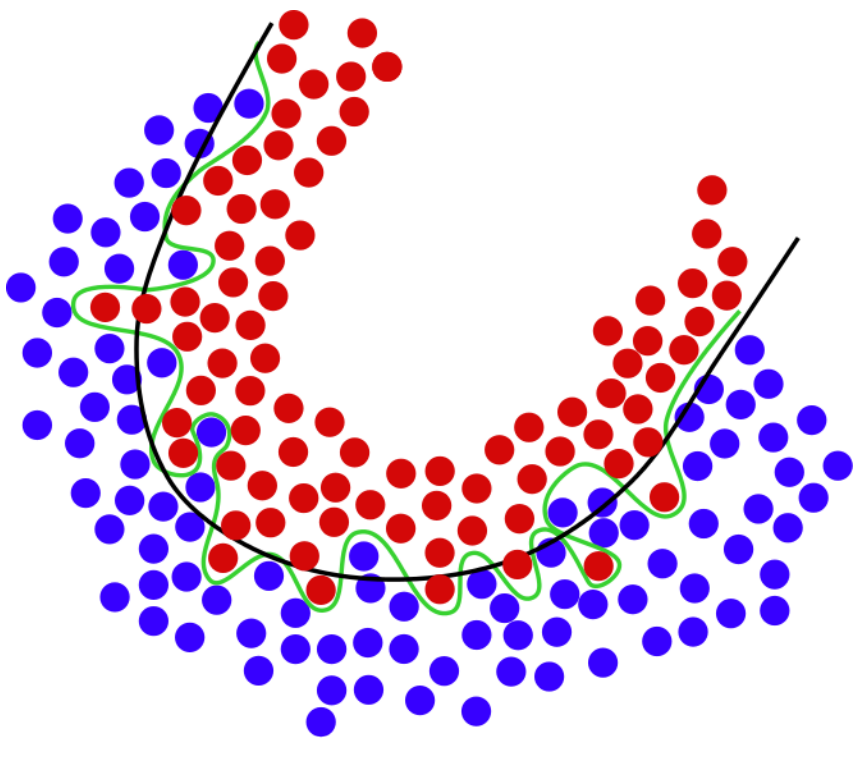
\includegraphics[width=0.5\textwidth]{chapter7/img/overtraining.png}
\caption{Example of overtraining. In black, the theoretical line between background (blue points) and signal (red points) is given. An overtrained BDT will have a (perfect) selection such as the green line. Illustration from \cite{boserpdf}.}
\label{fig:overtraining}
\end{figure}

\subsubsection{Pruning}
\label{subsub:pruning}
The problem with overtraining is essentially that there are certain splits in a classifier tree that are too specific and less important. In the method of \textit{cost complexity pruning}, for each node the complexity is calculated as

\begin{equation}
\rho = \frac{\Delta S}{n_{\textrm{leaves}} -1},
\end{equation}
\noindent with $\Delta S$ the separation gain as defined in Eq. \ref{eq:separationgain}. The subtree of the node with the smallest value of $\rho$ is removed and this is done repeatedly until a desired \textit{pruning strength}\footnote{A parameter on a scale from 0 to 100, which specifies the percentage of the pruning sequence to actually execute. 0 means no pruning is done and 100 signifies only a single root node remaining.} is reached.\\
\newline
\noindent BDTs are always trained and tested with different subsets of the same type (background or signal) of event. If the training set has significantly different scores than the testing set, the sample is most probably overtrained and one has to change the BDT input parameters. Typically, one uses Kolmogorov-Smirnov testing to indicate if the BDT score distributions from the training and testing sets could follow the same distribution pattern. As a rule of thumb, a $p_{KS} \lesssim 0.01$ indicates overtraining beyond the level of comfort.


\subsubsection{Data-MC agreement}
\textcolor{red}{Nodig?}	

\section{Minimal-Redundancy-Maximum-Relevance}
\label{sec:mrmr}
Having multiple variables that are able to discriminate signal from background events is a neccesary tool to ensure to conclude statements about a certain theory or exotic phenomenon. Single variables can show promising results, but when multiple variables are highly correlated much of the discriminative power diminishes. When using BDTs, analyzers often try to include variables and remove them if they show to be highly correlated in a trial-and-error fashion.

In this analysis, I made use of a technique that was originally developed for data in biological sciences but can be used for most analyses that involve ``data mining ''. Variables from a large sample set were selected with the condition of minimal-Redundancy-Maximal-Relevance (mRMR). To optimize the characterization of a certain class of events with a set of variables, these variables are selected with a \textit{maximal relevance}. ``Relevance'' is characterized in terms of correlation of mutual information. Because combinations of individually good features do not necessarily lead to good classification performance, there is the additional requirement of \textit{minimal redundancy} \cite{1453511}.\\

\noindent In this analysis, mRMR was used to rank variables from a large set according to their importance and proved to lead to low correlated variables (see Fig. ???).

